% Options for packages loaded elsewhere
\PassOptionsToPackage{unicode}{hyperref}
\PassOptionsToPackage{hyphens}{url}
\PassOptionsToPackage{dvipsnames,svgnames,x11names}{xcolor}
%
\documentclass[
  11pt,
  letterpaper,
]{article}

\usepackage{amsmath,amssymb}
\usepackage{iftex}
\ifPDFTeX
  \usepackage[T1]{fontenc}
  \usepackage[utf8]{inputenc}
  \usepackage{textcomp} % provide euro and other symbols
\else % if luatex or xetex
  \usepackage{unicode-math}
  \defaultfontfeatures{Scale=MatchLowercase}
  \defaultfontfeatures[\rmfamily]{Ligatures=TeX,Scale=1}
\fi
\usepackage{lmodern}
\ifPDFTeX\else  
    % xetex/luatex font selection
\fi
% Use upquote if available, for straight quotes in verbatim environments
\IfFileExists{upquote.sty}{\usepackage{upquote}}{}
\IfFileExists{microtype.sty}{% use microtype if available
  \usepackage[]{microtype}
  \UseMicrotypeSet[protrusion]{basicmath} % disable protrusion for tt fonts
}{}
\makeatletter
\@ifundefined{KOMAClassName}{% if non-KOMA class
  \IfFileExists{parskip.sty}{%
    \usepackage{parskip}
  }{% else
    \setlength{\parindent}{0pt}
    \setlength{\parskip}{6pt plus 2pt minus 1pt}}
}{% if KOMA class
  \KOMAoptions{parskip=half}}
\makeatother
\usepackage{xcolor}
\usepackage[margin=1in]{geometry}
\setlength{\emergencystretch}{3em} % prevent overfull lines
\setcounter{secnumdepth}{5}
% Make \paragraph and \subparagraph free-standing
\ifx\paragraph\undefined\else
  \let\oldparagraph\paragraph
  \renewcommand{\paragraph}[1]{\oldparagraph{#1}\mbox{}}
\fi
\ifx\subparagraph\undefined\else
  \let\oldsubparagraph\subparagraph
  \renewcommand{\subparagraph}[1]{\oldsubparagraph{#1}\mbox{}}
\fi


\providecommand{\tightlist}{%
  \setlength{\itemsep}{0pt}\setlength{\parskip}{0pt}}\usepackage{longtable,booktabs,array}
\usepackage{calc} % for calculating minipage widths
% Correct order of tables after \paragraph or \subparagraph
\usepackage{etoolbox}
\makeatletter
\patchcmd\longtable{\par}{\if@noskipsec\mbox{}\fi\par}{}{}
\makeatother
% Allow footnotes in longtable head/foot
\IfFileExists{footnotehyper.sty}{\usepackage{footnotehyper}}{\usepackage{footnote}}
\makesavenoteenv{longtable}
\usepackage{graphicx}
\makeatletter
\def\maxwidth{\ifdim\Gin@nat@width>\linewidth\linewidth\else\Gin@nat@width\fi}
\def\maxheight{\ifdim\Gin@nat@height>\textheight\textheight\else\Gin@nat@height\fi}
\makeatother
% Scale images if necessary, so that they will not overflow the page
% margins by default, and it is still possible to overwrite the defaults
% using explicit options in \includegraphics[width, height, ...]{}
\setkeys{Gin}{width=\maxwidth,height=\maxheight,keepaspectratio}
% Set default figure placement to htbp
\makeatletter
\def\fps@figure{htbp}
\makeatother
\newlength{\cslhangindent}
\setlength{\cslhangindent}{1.5em}
\newlength{\csllabelwidth}
\setlength{\csllabelwidth}{3em}
\newlength{\cslentryspacingunit} % times entry-spacing
\setlength{\cslentryspacingunit}{\parskip}
\newenvironment{CSLReferences}[2] % #1 hanging-ident, #2 entry spacing
 {% don't indent paragraphs
  \setlength{\parindent}{0pt}
  % turn on hanging indent if param 1 is 1
  \ifodd #1
  \let\oldpar\par
  \def\par{\hangindent=\cslhangindent\oldpar}
  \fi
  % set entry spacing
  \setlength{\parskip}{#2\cslentryspacingunit}
 }%
 {}
\usepackage{calc}
\newcommand{\CSLBlock}[1]{#1\hfill\break}
\newcommand{\CSLLeftMargin}[1]{\parbox[t]{\csllabelwidth}{#1}}
\newcommand{\CSLRightInline}[1]{\parbox[t]{\linewidth - \csllabelwidth}{#1}\break}
\newcommand{\CSLIndent}[1]{\hspace{\cslhangindent}#1}

\usepackage{amsfonts}
\DeclareMathAlphabet{\mathams}{U}{msb}{m}{n}
\usepackage{algorithm}
\usepackage{algpseudocode}
\usepackage{setspace}
\doublespacing
\makeatletter
\makeatother
\makeatletter
\makeatother
\makeatletter
\@ifpackageloaded{caption}{}{\usepackage{caption}}
\AtBeginDocument{%
\ifdefined\contentsname
  \renewcommand*\contentsname{Table of contents}
\else
  \newcommand\contentsname{Table of contents}
\fi
\ifdefined\listfigurename
  \renewcommand*\listfigurename{List of Figures}
\else
  \newcommand\listfigurename{List of Figures}
\fi
\ifdefined\listtablename
  \renewcommand*\listtablename{List of Tables}
\else
  \newcommand\listtablename{List of Tables}
\fi
\ifdefined\figurename
  \renewcommand*\figurename{Figure}
\else
  \newcommand\figurename{Figure}
\fi
\ifdefined\tablename
  \renewcommand*\tablename{Table}
\else
  \newcommand\tablename{Table}
\fi
}
\@ifpackageloaded{float}{}{\usepackage{float}}
\floatstyle{ruled}
\@ifundefined{c@chapter}{\newfloat{codelisting}{h}{lop}}{\newfloat{codelisting}{h}{lop}[chapter]}
\floatname{codelisting}{Listing}
\newcommand*\listoflistings{\listof{codelisting}{List of Listings}}
\makeatother
\makeatletter
\@ifpackageloaded{caption}{}{\usepackage{caption}}
\@ifpackageloaded{subcaption}{}{\usepackage{subcaption}}
\makeatother
\makeatletter
\@ifpackageloaded{tcolorbox}{}{\usepackage[skins,breakable]{tcolorbox}}
\makeatother
\makeatletter
\@ifundefined{shadecolor}{\definecolor{shadecolor}{rgb}{.97, .97, .97}}
\makeatother
\makeatletter
\makeatother
\makeatletter
\makeatother
\ifLuaTeX
  \usepackage{selnolig}  % disable illegal ligatures
\fi
\IfFileExists{bookmark.sty}{\usepackage{bookmark}}{\usepackage{hyperref}}
\IfFileExists{xurl.sty}{\usepackage{xurl}}{} % add URL line breaks if available
\urlstyle{same} % disable monospaced font for URLs
\hypersetup{
  pdftitle={A Review of Methods for Explainable and Interpretable Graph Neural Networks},
  pdfauthor={Art Tay},
  colorlinks=true,
  linkcolor={blue},
  filecolor={Maroon},
  citecolor={Blue},
  urlcolor={Blue},
  pdfcreator={LaTeX via pandoc}}

\title{A Review of Methods for Explainable and Interpretable Graph
Neural Networks}
\author{Art Tay}
\date{}

\begin{document}
\maketitle
\ifdefined\Shaded\renewenvironment{Shaded}{\begin{tcolorbox}[frame hidden, enhanced, borderline west={3pt}{0pt}{shadecolor}, sharp corners, boxrule=0pt, breakable, interior hidden]}{\end{tcolorbox}}\fi

\hypertarget{introduction}{%
\section{Introduction}\label{introduction}}

\quad Graphs provide an incredibly flexible structure for modeling
complex data. Data can naturally appear as graphs, like molecules. We
can reduce data to a graph, such as the key points of a image. We can
even use graphs to add structure, such as grammatical relationships.
Graph Neural Networks (GNNs) have become a popular choice for prediction
and inference on graph data. At their core, GNNs work by iteratively
updating node embeddings based on information from neighboring nodes.
The idea is to use the graph's structure to engineer better features.
This message passing scheme allows GNNs to capture complex dependencies
and patterns present within the graph structure. GNN architectures
typically consist of multiple layers, each performing message passing
and aggregation operations to refine the embeddings. These layers are
often followed by pooling and dense prediction layers to produce the
final output. Some important applications of graph classification
include predicting chemical toxicity
(\protect\hyperlink{ref-bai2019unsupervised}{Bai et al. 2019}),
classifying proteins
(\protect\hyperlink{ref-gallicchio2019fast}{Gallicchio and Micheli
2019}), and even detecting cancer from pathology slides
(\protect\hyperlink{ref-Xiao_Wang_Rong_Yang_Zhang_Zhan_Bishop_Wilhelm_Zhang_Pickering_et_al._2023}{Xiao
et al. 2023}). While GNNs achieve remarkable predictive power, their
complexity prevents the exaction of the scientific rationale. Like many
deep learning models, the black box nature of GNNs prevents wide
adoption. Without strong methods for understanding their predictions,
GNNs are more susceptible to adversarial attacks and undetected
discrimination. Inferential methods also serve to direct modeling
efforts by highlighting common structures or features that may be
predictive in other applications. These reasons underscore the critical
importance of methods for explaining and interpreting GNN models.

\quad Although explainability and interpretability are sometimes used
interchangeably in the literature, we will adopt the distinction
expressed in Yuan et al.
(\protect\hyperlink{ref-Yuan_Yu_Gui_Ji_2022}{2022}). In this article the
authors say that a model is explainable if the models predictions can be
reasoned post-hoc (\protect\hyperlink{ref-Yuan_Yu_Gui_Ji_2022}{Yuan et
al. 2022}). For example, the effect of a specific input variable can be
estimated by either dropping or randomly permuting the variable and
accessing the effect on the output
(\protect\hyperlink{ref-Breiman_2001}{Breiman 2001}). This paradigm
could be directly applied to GNNs; however, researchers are often not
interested in the statistical significance of tabular node and
edge-level features. Most scientific questions focus on the importance
of specific graph-level substructures. The challenge with GNN
explanations is that, in addition to computing the importance of
features, the high-level features themselves must first be identified.
On the other hand, a model is interpretable if the model's decision
process can be readily understood by humans
(\protect\hyperlink{ref-Yuan_Yu_Gui_Ji_2022}{Yuan et al. 2022}). For
example, a linear regression model is interpretable because each
coefficient clearly defines the relationship between any input and
output. An interpretable model is typically superior to an explainable
one because similar to a partial F-test, explanation methods might
identify that certain variables enhance the model, but they cannot
explain how these variables contribute. On the flip side, interpretable
models may not reach the performance levels of black-box models. GNN
models are generally not interpretable because the relation expressed by
the parameters tends to exceed human understanding. A direct translation
from traditional statistics would be a circuit type analysis, which has
work for image processing convolution neural networks
(\protect\hyperlink{ref-olah2020zoom}{Olah et al. 2020}). For graphs,
this would involve using coefficients on subgraphs to produce
predictions. Similar to the difficulties of explanation methods, these
subgraphs would have to be identified, which can be computational
complex and expensive given the combinatorial nature of graphs.
Overcoming these challenges has substantial scientific impacts. In
applications where GNNs demonstrate strong predictive power, it enables
the formulation of testable scientific hypotheses about the nature of
the classification. Conversely, in cases where GNNs exhibit weak
predictive power, it helps identify and understand potential
misunderstandings within the model.

\hypertarget{general-notation}{%
\subsection{General Notation}\label{general-notation}}

\begin{itemize}
\item
  Any graph \(G\) can be describe by \(X, A, E\). The node feature,
  matrix, edge feature matrix, and adjacency matrix respectively.
\item
  Let \(X = [X_c, \ X_d]\), where \(X_c\) is the subset of continuous
  node features and \(X_d\) is the subset of one-hot discrete node
  features.
\item
  Let \(E = [E_c, \ E_d]\), denoted in the same manner.
\item
  Let \(n\) represent the number of nodes in the graph and \(v\)
  represent the number of edges.
\item
  For any graph, let \(\nu\) denote the set of node and \(\mathcal{E}\)
  denote the set of edges.
\item
  Let \(\text{feat}_{(.)}\) denote the number of features or columns in
  the the corresponding feature matrix.
\item
  \(A\) is a binary \(n \times n\) matrix where \(A[i, \ j] = 1\)
  indicates that an edge exists between nodes labeled \(i\) and \(j\).
\item
  Let
  \(\text{explainee}(G; \ \Omega) = h^{(1)}_G, \dots h^{(L)}_G, \rho_G\)
  be an \(L\) layer GNN model with parameters \(\Omega\) that we would
  like to explain.
\item
  Let \(\hat Y_G\) be the predicted class label for graph \(G\)
  predicted from explainee().
\item
  Unless otherwise noted, assume any GNN model discussed is a
  graph-level classification model.
\end{itemize}

\hypertarget{analysis-of-core-papers}{%
\section{Analysis of Core Papers}\label{analysis-of-core-papers}}

\hypertarget{gnninterpreter-wang_shen_2024}{%
\subsection{\texorpdfstring{GNNInterpreter
(\protect\hyperlink{ref-Wang_Shen_2024}{Wang and Shen
2024})}{GNNInterpreter (Wang and Shen 2024)}}\label{gnninterpreter-wang_shen_2024}}

\quad GNNInterpreter (\protect\hyperlink{ref-Wang_Shen_2024}{Wang and
Shen 2024}) is a method for generating model-level explanations of GNN
graph classification models. In general, explanation methods serve to
elucidate which features within the data influence disparate
predictions. These methods typically fall into two categories:
instance-level and model-level. Instance-level explanations aim to
unveil the model's rationale behind a particular prediction. In domains
such as image and text analysis, a prevalent approach involves masking
or perturbing the instance and assessing the impact on the model's
prediction. On the other hand, model-level explanations seek to
understand how a model generally distinguishes between classes. In image
and text analysis, for instance, one common technique involves treating
the input as a trainable parameter and optimizing the model's prediction
towards a specific class. Consequently, the resulting optimized input
comprises a set of features strongly associated with the targeted class.
GNNInterpreter provides model level explanations for GNN in this manner.
Formally, GNNInterpreter tries to learn the graph generating
distribution for each class. GNNInterpreter works by optimizing the
parameters of a generic graph generating distribution to produce samples
that closely match the explainee's understanding of the targeted class.

\quad Graph generating distributions are hard to specify because there
can be discrete and continuous elements of \(X\), \(E\) and \(A\).
Furthermore, the interactions between these matrices can be complex. The
authors tackle these issues by making two simplify assumptions. First,
they assume that every graph is a \emph{Gilbert random graph}
(\protect\hyperlink{ref-Gilbert_1959}{Gilbert 1959}), where every
possible edge as an independent fixed probability of occurring. Second,
the author assume that the features of every node and edge are
independently distributed. The justification of the first assumption is
that the other common types of random graphs are not suitable for this
application. Erdo-Renyi random graphs
(\protect\hyperlink{ref-erdds1959random}{ERDdS and R\&wi 1959}) have a
fixed number of edges, which limits the diversity of explanations, Rado
random graphs (\protect\hyperlink{ref-Rado1964UniversalGA}{Rado 1964})
are infinite in size, and the random dot-product graph model is just a
generalization of Gilbert's model. The second assumption is justified by
the fact that the parameters of the independent distributions will be
updated jointly using the \emph{explainee} model. Therefore, the
\emph{explainee's} understanding of the latent correlation structure
should be contained in the final estimates.

\quad Although the graphs discuss in this paper only contain discrete
features, \(X_c\) and \(E_c\) can be sampled from any continuous
distribution that can be expressed as a location-scale family.
Separating the stochastic and systematic components is necessary for
gradient based optimization. It is commonly known as the
\emph{reparametrization trick}. The discrete feature matrices, (\(X_d\),
\(E_d\), \(A\)), need to be sampled from a continuous distribution for
gradient based optimization, but the distribution has to have sampling
properties close to a discrete distribution. The author assume that the
true underlying distribution for every discrete node and edge feature is
\emph{categorical}. The categorical distribution is also know as the
multi-bernoulli, where every sample has a fixed probability of being in
one of the discrete categories. Let \(\theta_\text{cat}\) represent the
associated vector of un-normalized or relative probabilities, where each
entries is \(>0\). Then,

\begin{equation} \label{gumbel-max-eq}
    \text{argmax} \ \log \theta_\text{cat} + \text{Gumbel}(0, 1)
        \sim \text{Cat}(\theta_\text{cat})
\end{equation}

The intuition is that the Gumbel distribution, which is the density of
the maximum order statistic of i.i.d. standard normals, makes it a good
candidate for modeling the winning or maximum probability category.
Adding Gumbel noise to the logits should maintain the true relative
proportions, but enough skewness such that every category has some
probability of having the maximum noised logit. A proof of equation
\ref{gumbel-max-eq} is provide in section Section~\ref{sec-proof}.
Approximating the argmax function with the Softmax function allows for
approximate categorical sampling that is differentiable w.r.t.
\(\theta_\text{cat}\). The associate inverse uniform CDF sampling
formula below is referred to as the \emph{Gumbel-Softmax trick} or the
\emph{concrete distribution}
(\protect\hyperlink{ref-Maddison_Mnih_Teh_2017}{Maddison, Mnih, and Teh
2017}). \begin{equation}
    \text{Softmax}
    \left(
        \dfrac{\log \theta_{\text{Cat}} - log(-log \ \epsilon)}{\tau}
    \right), \quad \epsilon \sim U[0, 1].
\end{equation} \(\tau\) is a hyperparameter that controls the degree of
relaxation. Smaller value of \(\tau\) approximate the discrete sampling
better, but can result in numerical issues. The adjacency matrix can be
sampled in a similar manner since the Bernoulli is just a special case
of the categorical.\\
\begin{equation} \label{binary-concrete}
        \text{sigmoid}
            \left(\dfrac{\log(\theta_A / (1 - \theta_A)) + \log \ \epsilon - \log(1 - \log \ \epsilon)}{\tau} \right), \quad \epsilon \sim U[0, 1], 
    \end{equation} where \(\theta_A\) is an \(n \times n\) matrix with
each \([i, j]\) entry representing the relative probability that the
\(ij\) edge exists. Equation \ref{binary-concrete} samples from the
binary concrete distribution
(\protect\hyperlink{ref-Maddison_Mnih_Teh_2017}{Maddison, Mnih, and Teh
2017}). Taken together, let\\
\[
    G_{\text{gen}} \sim \text{gen}(\Theta)  
\]

notate the combined graph generating distribution, where \(\Theta\) is
the set of all parameters from the independently sampled distributions.

\quad An obvious objective is to maximize the likelihood that the
\emph{explainee} model predicts a sampled graph to be a member of the
target class. Let \(\tilde{\rho}\) denote the desired predicted
probability vector. Then the above objective can be expressed as:
\begin{equation}
        \mathcal{L}_\text{pred} (\Theta \ | \ G_\text{gen}) = \mathams{E}_{G_\text{gen}} \ \text{CrtEnt} (\text{explainee}(G_\text{gen}), \ \tilde{\rho})
    \end{equation} While the above objective enforces a desirable
property, it fails to be restrictive enough to generate realistic
graphs. This is because the final prediction, \(\rho_{G_{\text{gen}}}\)
is compute using only final embeddings, \(h^{(L)}_{G_{\text{gen}}}\).
Normally \(h^{(L)}_{G_{\text{gen}}}\) contains all the needed
information from the graphs structure; however, the generation scheme
allows the feature distribution to be optimized directly. This means
that an explanation can ignore the graph structure and optimize towards
the desired final embeddings. It is dangerously common for nonsensical
features and structures at the graph level to end up on the desired side
of the decision boundary. Empirically, the authors found that even
completely random graphs can produce confidence and consistent
predictions.

\begin{figure}

{\centering 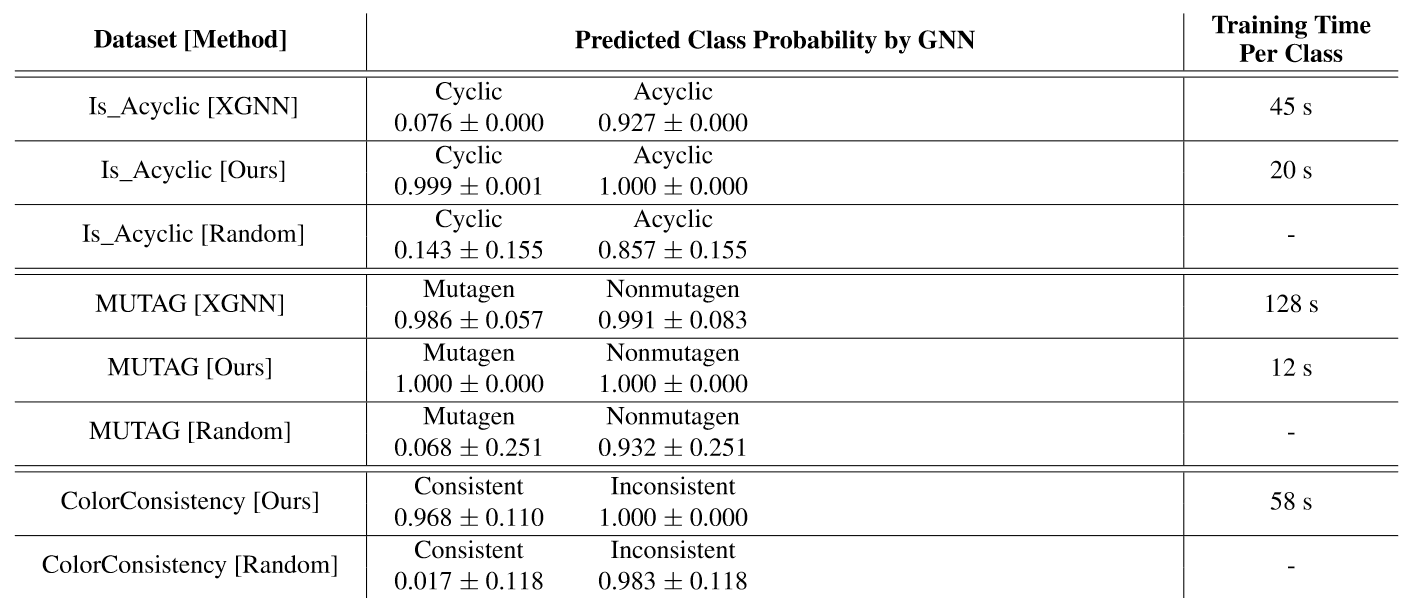
\includegraphics{figures/random_baseline.png}

}

\caption{\label{fig-random-baseline}An abridged copy of Table 5 from
Wang and Shen (\protect\hyperlink{ref-Wang_Shen_2024}{2024}).}

\end{figure}

For example, Figure~\ref{fig-random-baseline} shows that random graphs
had an average predicted probability of being non-mutagenic in the MUTAG
dataset (\protect\hyperlink{ref-Debnath_1991}{Debnath et al. 1991}) if
93.2\%. In order to mitigate this issue, the authors proposed additional
minimizing the cosine distance between the average embedding of all the
observed graph from the targeted class, \(\bar h^{(L)}_{G_c}\), and the
embedding of the generated explanation: \begin{equation}
       \mathcal{L}_{\text{embed}}(\Theta \ | \ G_\text{gen}) = 
            \mathams{E}_{G_\text{gen}}
            \text{CosDist}\left( \bar h^{(L)}_{G_c}, \ h^{(L)}_{G_\text{gen}} \right). 
    \end{equation}

\hypertarget{d4explainer-chen_wu_gupta_ying_2023}{%
\subsection{\texorpdfstring{D4Explainer
(\protect\hyperlink{ref-Chen_Wu_Gupta_Ying_2023}{Chen et al.
2023})}{D4Explainer (Chen et al. 2023)}}\label{d4explainer-chen_wu_gupta_ying_2023}}

\hypertarget{protgnn-zhang_liu_wang_lu_lee_2021}{%
\subsection{\texorpdfstring{ProtGNN
(\protect\hyperlink{ref-Zhang_Liu_Wang_Lu_Lee_2021}{Zhang et al.
2021})}{ProtGNN (Zhang et al. 2021)}}\label{protgnn-zhang_liu_wang_lu_lee_2021}}

\hypertarget{synthesis-of-core-papers}{%
\section{Synthesis of Core Papers}\label{synthesis-of-core-papers}}

\hypertarget{technical-details}{%
\section{Technical Details}\label{technical-details}}

\hypertarget{methodology}{%
\subsection{Methodology}\label{methodology}}

\hypertarget{results}{%
\subsection{Results}\label{results}}

\hypertarget{sec-proof}{%
\subsection{Proofs}\label{sec-proof}}

\textbf{Proof of Equation \ref{gumbel-max-eq}:} WLOG assume we want to
sample for a categorical distribution \(\text{cat}(\theta_\text{cat})\)
with a set of \(W\) categories each with a probability \[
\pi_\omega = \dfrac{\theta_\text{cat}[\omega]}{\sum_{i \in W}\theta_\text{cat}[i]}.
\]

Define random variable \[
D = \text{argmax} \ \log \theta_\text{cat} + \text{Gumbel}(0, 1) = \underset{i \in W}{\text{argmax}} \ \log \theta_\text{cat}[i] + \text{Gumbel}(0, 1)[i], 
\]

here \(\text{Gumbel}(0, 1)[i]\) denotes the \(i^{th}\) i.i.d. sample
from the associated Gumbel. In order for \(D\) to be a true categorical
random variable, \(Pr[D = \omega]\) need to be \(\pi_\omega\).
\(D = \omega\) if and only if
\(\log \theta_\text{cat}[\omega] + \text{Gumbel}(0,1)[\omega] > \log \theta_\text{cat}[i] + \text{Gumbel}(0, 1)[i] \ \forall i \in W \setminus \omega\).
Now, let \(M_i\) denote a random variable that follows a
\(\text{Gumbel}(\log \theta_\text{cat}[i], 1)\) distribution. Then,
\begin{align*}
        Pr[D = \omega] 
            &= \mathams{E}_{M_\omega} 
                \prod_{i \in W \setminus \omega} Pr(M_i < m_\omega) 
                \text{ i.i.d location shifted Gumbel distributions.} \\ 
            &= \mathams{E}_{M_\omega} 
                \prod_{i \in W \setminus \omega} \exp 
                    \left(-e^{\log \theta_\text{cat}[i] - m_\omega} \right)
                \text{ Gumbel CDF.} \\ 
            &= \mathams{E}_{M_\omega} 
                \exp \left(-\sum_{i \in W \setminus \omega}
                e^{\log \theta_\text{cat}[i] - m_\omega} \right) \\ 
            &= \int_{-\infty}^{\infty}
                \exp \left( \log \theta_\text{cat}[\omega] - m_\omega \right) 
                \exp \left(-e^{\log \theta_\text{cat}[\omega] - m_\omega} \right) \cdot 
                \exp \left (-\sum_{i \in W \setminus \omega}
                e^{\log \theta_\text{cat}[i] - m_\omega} \right) \ dm \\
                &\text{ Gumbel PDF.} \\
            &= \int_{-\infty}^{\infty}
                \exp \left( \log \theta_\text{cat}[\omega] - m_\omega \right) 
                \exp \left (-\sum_{i \in W}
                e^{\log \theta_\text{cat}[i] - m_\omega} \right) \ dm \\
            &= \int_{-\infty}^{\infty}
                \theta_\text{cat}[\omega] 
                \exp \left( -m_\omega \right) 
                \exp \left( -e^{-m_\omega} \sum_{i \in W}
                    \theta_\text{cat}[i]  \right) \ dm \\
            &= \pi_\omega \sum_{i \in W} \theta_\text{cat}[i]
            \int_{-\infty}^{\infty}
                \exp \left( -m_\omega \right) 
                \exp \left( -e^{-m_\omega} \sum_{i \in W}
                    \theta_\text{cat}[i]  \right) \ dm 
                    \text{ From the above definition of } \pi_\omega \\
            &= \pi_\omega \sum_{i \in W} \theta_\text{cat}[i]
                \dfrac{\exp\left( -e^{-m_\omega} \sum_{i \in W} \theta_\text{cat}[i] \right)
                    }{\sum_{i \in W} \theta_\text{cat}[i]} \bigg|_{-\infty}^\infty \\ 
            &= \pi_\omega \sum_{i \in W} \theta_\text{cat}[i]
                \dfrac{1}{\sum_{i \in W} \theta_\text{cat}[i]} = \pi_\omega. 
    \end{align*} Reference: Huijben et al.
(\protect\hyperlink{ref-Huijben_Kool_Paulus_van_Sloun_2022}{2022})

\hypertarget{future-directions}{%
\section{Future Directions}\label{future-directions}}

\pagebreak

\hypertarget{references}{%
\section{References}\label{references}}

\hypertarget{refs}{}
\begin{CSLReferences}{1}{0}
\leavevmode\vadjust pre{\hypertarget{ref-bai2019unsupervised}{}}%
Bai, Yunsheng, Hao Ding, Yang Qiao, Agustin Marinovic, Ken Gu, Ting
Chen, Yizhou Sun, and Wei Wang. 2019. {``Unsupervised Inductive
Graph-Level Representation Learning via Graph-Graph Proximity.''}
\url{https://arxiv.org/abs/1904.01098}.

\leavevmode\vadjust pre{\hypertarget{ref-Breiman_2001}{}}%
Breiman, Leo. 2001. {``Random Forests.''} \emph{Machine Learning} 45
(1): 5--32. \url{https://doi.org/10.1023/A:1010933404324}.

\leavevmode\vadjust pre{\hypertarget{ref-Chen_Wu_Gupta_Ying_2023}{}}%
Chen, Jialin, Shirley Wu, Abhijit Gupta, and Rex Ying. 2023.
{``D4Explainer: In-Distribution GNN Explanations via Discrete Denoising
Diffusion,''} no. arXiv:2310.19321 (October).
\url{https://doi.org/10.48550/arXiv.2310.19321}.

\leavevmode\vadjust pre{\hypertarget{ref-Debnath_1991}{}}%
Debnath, Asim Kumar, Rosa L. Lopez de Compadre, Gargi Debnath, Alan J.
Shusterman, and Corwin Hansch. 1991. {``Structure-Activity Relationship
of Mutagenic Aromatic and Heteroaromatic Nitro Compounds. Correlation
with Molecular Orbital Energies and Hydrophobicity.''} \emph{Journal of
Medicinal Chemistry} 34 (2): 786--97.
\url{https://doi.org/10.1021/jm00106a046}.

\leavevmode\vadjust pre{\hypertarget{ref-erdds1959random}{}}%
ERDdS, P, and A R\&wi. 1959. {``On Random Graphs i.''} \emph{Publ. Math.
Debrecen} 6 (290-297): 18.

\leavevmode\vadjust pre{\hypertarget{ref-gallicchio2019fast}{}}%
Gallicchio, Claudio, and Alessio Micheli. 2019. {``Fast and Deep Graph
Neural Networks.''} \url{https://arxiv.org/abs/1911.08941}.

\leavevmode\vadjust pre{\hypertarget{ref-Gilbert_1959}{}}%
Gilbert, E. N. 1959. {``Random Graphs.''} \emph{The Annals of
Mathematical Statistics} 30 (4): 1141--44.

\leavevmode\vadjust pre{\hypertarget{ref-Huijben_Kool_Paulus_van_Sloun_2022}{}}%
Huijben, Iris A. M., Wouter Kool, Max B. Paulus, and Ruud J. G. van
Sloun. 2022. {``A Review of the Gumbel-Max Trick and Its Extensions for
Discrete Stochasticity in Machine Learning,''} no. arXiv:2110.01515
(March). \url{https://doi.org/10.48550/arXiv.2110.01515}.

\leavevmode\vadjust pre{\hypertarget{ref-Maddison_Mnih_Teh_2017}{}}%
Maddison, Chris J., Andriy Mnih, and Yee Whye Teh. 2017. {``The Concrete
Distribution: A Continuous Relaxation of Discrete Random Variables,''}
no. arXiv:1611.00712 (March).
\url{https://doi.org/10.48550/arXiv.1611.00712}.

\leavevmode\vadjust pre{\hypertarget{ref-olah2020zoom}{}}%
Olah, Chris, Nick Cammarata, Ludwig Schubert, Gabriel Goh, Michael
Petrov, and Shan Carter. 2020. {``Zoom in: An Introduction to
Circuits.''} \emph{Distill}.
\url{https://doi.org/10.23915/distill.00024.001}.

\leavevmode\vadjust pre{\hypertarget{ref-Rado1964UniversalGA}{}}%
Rado, Richard. 1964. {``Universal Graphs and Universal Functions.''}
\emph{Acta Arithmetica} 9: 331--40.
\url{https://api.semanticscholar.org/CorpusID:118279788}.

\leavevmode\vadjust pre{\hypertarget{ref-Wang_Shen_2024}{}}%
Wang, Xiaoqi, and Han-Wei Shen. 2024. {``GNNInterpreter: A Probabilistic
Generative Model-Level Explanation for Graph Neural Networks,''} no.
arXiv:2209.07924 (February).
\url{https://doi.org/10.48550/arXiv.2209.07924}.

\leavevmode\vadjust pre{\hypertarget{ref-Xiao_Wang_Rong_Yang_Zhang_Zhan_Bishop_Wilhelm_Zhang_Pickering_et_al._2023}{}}%
Xiao, Guanghua, Shidan Wang, Ruichen Rong, Donghan Yang, Xinyi Zhang,
Xiaowei Zhan, Justin Bishop, et al. 2023. \emph{Deep Learning of Cell
Spatial Organizations Identifies Clinically Relevant Insights in Tissue
Images}. Preprint. In Review.
\url{https://doi.org/10.21203/rs.3.rs-2928838/v1}.

\leavevmode\vadjust pre{\hypertarget{ref-Yuan_Yu_Gui_Ji_2022}{}}%
Yuan, Hao, Haiyang Yu, Shurui Gui, and Shuiwang Ji. 2022.
{``Explainability in Graph Neural Networks: A Taxonomic Survey,''} no.
arXiv:2012.15445 (July).
\url{https://doi.org/10.48550/arXiv.2012.15445}.

\leavevmode\vadjust pre{\hypertarget{ref-Zhang_Liu_Wang_Lu_Lee_2021}{}}%
Zhang, Zaixi, Qi Liu, Hao Wang, Chengqiang Lu, and Cheekong Lee. 2021.
{``ProtGNN: Towards Self-Explaining Graph Neural Networks,''} no.
arXiv:2112.00911 (December).
\url{https://doi.org/10.48550/arXiv.2112.00911}.

\end{CSLReferences}

\hypertarget{appendix}{%
\section{Appendix}\label{appendix}}



\end{document}
